\documentclass[a4paper, 11pt]{article}
\usepackage[utf8]{inputenc}
\usepackage{hyperref}
\usepackage[arrowdel]{physics}
\usepackage[swedish]{babel}
\usepackage{graphicx}

\newcommand{\vect}[1]{\vectorbold{#1}}
\newcommand{\deriv}{\subparagraph{Härledning}}
\renewcommand{\Re}[1]{\operatorname{Re}\left(#1\right)}

\title{Sammanfattning av SK1104}
\author{Yashar Honarmandi}
\date{\today}

\begin{document}\sloppy

\maketitle

\begin{abstract}
	Detta ær en sammanfattning av kursen SH1014 Modern fysik.
\end{abstract}

\pagenumbering{roman}
\thispagestyle{empty}

\newpage

\tableofcontents

\newpage

\pagenumbering{arabic}

\section{Notation}
Om inte annat specifieras, kommer alla ekvationer använda notationen som ges i denna tabellen.

\begin{table}[!h]
	\centering
	\begin{tabular}{| l | c |}
		\hline
		\textbf{Storhet} & \multicolumn{1}{|l|}{\textbf{Symbol}}\\
		Position         & $\vect{r}$ \\
		\hline
		Tid              & $t$ \\
		\hline
		Period           & $T$ \\
		\hline
		Frekvens         & $f$ \\
		\hline
		Vinkelfrekvens   & $\omega$ \\
		\hline
		Våglängd         & $\lambda$ \\
		\hline
		Vågvektor        & $\vect{k}$ \\
		\hline
		Vågtal           & $k$ \\
		\hline
		Amplitud         & $A$ \\
		\hline
		Vågfart          & $c$ \\
		\hline
	\end{tabular}
\end{table}

\section{Harmoniska vågor}
Harmoniska vågor, även kallad plana vågor, är periodiska störningar i ett medium, och beskrivs typisk av en funktion på formen $e^{i\phi}$. För dessa kan man identifiera vissa storheter, somm vi kommer göra här.

\paragraph{Perioden}
Perioden är tiden det tar för en harmonisk våg att gå genom en cykel.

\paragraph{Frekvens och vinkelfrekvens}
Av större intresse är frekvens, som ges av
\begin{align*}
	f = \frac{1}{T},
\end{align*}
som då är antalet cykler vågen går genom per enhet tid. Av ännu större intresse är vinkelfrekvensen, som ges av
\begin{align*}
	\omega = 2\pi f = \frac{2\pi}{T},
\end{align*}
och ger antalet radianer vågen går genom per enhet tid.

\paragraph{Våglängd}
Våglängden är det minsta avståndet mellan två punkter som är i fas.

\paragraph{Vågvektor och vågtal}
För vågor i flera dimensioner är det smartare att använda en vågvektor. Denna har riktning motsvarande riktningen vågen propagerar i och längd
\begin{align*}
	k = \frac{2\pi}{\lambda}.
\end{align*}
$k$ kallas även vågtalet. Anledningen till att man heller använder vågvektorn är exakt den samma som att man heller använder frekvens än period.

\paragraph{Amplitud}
Harmoniska vågor representerar periodiska störningar. Denna störningen uppnår vid vissa tider ett maxvärde. Detta är vågens amplitud.

\section{Klassiska vågor}

\subsection{Principer}

\paragraph{Superposition}
Eftersom vågekvationen är linjär, interagerar vågor vid att man adderar störningarna.

\paragraph{Vågor i fas}
Två vågor är i fas om de har en fasskillnad lika med ett heltalsmultippel av $2\pi$.

\paragraph{Koherenta vågor}
Två vågor är koherenta om de har konstant fasskillnad.

\paragraph{Stående vågor}
En stående våg bildas när en våg reflekteras och interfererar med sig själv. En sådan våg har inten netto transport av energi.

\paragraph{Resonans}
Om en yttre kraft driver en svängning med en frekvens som naturligt ger stående vågor, växer amplituden obegränsat och man får stående vågor.

\paragraph{Fermats princip}
Strålgången till en klassisk våg mellan två punkter följer den snabbaste vägen.

\paragraph{Huygens' princip}
Om en våg utbrigdar sig i ett medium, kan varje punkt i mediet anses som en ny vågkälla som skickar ut en ny våg när den ursprungliga vågen träffer den givna punkten.

\paragraph{Rayleighs upplösningskriterium}
Två föremål är nätt och jämnt upplösta då interferensmaximum från det ena föremålet ligger i första sidominimum från det andra föremålet.

\subsection{Ekvationer}

\paragraph{Vågekvationen}
\begin{align*}
	\laplacian{s} = \frac{1}{c^2}\dv[2]{s}{t}
\end{align*}
Vågekvationen är fellesnämnaren för alla klassiska vågfenomen. Denna ekvation beskriver hur vågor med en väldefinierad fart $c$ propagerar i rymden över tid. $s$ är storheten som propagerar, t.ex. en tryckskillnad eller ett elektromagnetiskt fält.

\deriv
Låt störningen vara någon $f(\vect{n}\cdot\vect{r} - ct)$, der $\vect{n}$ är en enhetsvektor i samma riktning som vågens utbredning. $f$ har denna formen eftersom vågen efter en tid $t$ ser likadan ut om man beveger sig ett avstånd $ct$ i riktning av vågens utbredning. Med $u = \vect{n}\cdot\vect{r} - ct$ får man
\begin{align*}
	&\dv[2]{s}{x} = \dv{}{x}\dv{f}{u}\dv{u}{x} = n_x^2\dv[2]{f}{u}, \\
	&\vdots \\
	&\dv[2]{s}{t} = \dv{}{x}\dv{f}{u}\dv{u}{t} = c^2\dv[2]{f}{x}.
\end{align*}
Om man adderar derivatorna med avseende på rymdliga koordinater får man
\begin{align*}
	\laplacian{s} = \sum &\dv[2]{s}{x_i} = \sum n_i^2\dv[2]{f}{u} = \dv[2]{f}{u}\sum n_i^2 = \dv[2]{f}{u}
\end{align*}
då $\vect{n}$ är en enhetsvektor. Detta ger då
\begin{align*}
	\laplacian{s} = \frac{1}{c^2}\dv[2]{s}{t}.
\end{align*}

\paragraph{Dispersionsrelation för harmoniska vågor}
\begin{align*}
	\omega = ck
\end{align*}

\deriv
Ta en harmonisk våg i en dimension, på formen $Ae^{i(kx - \omega t)}$, och testa om den uppfyller vågekvationen. Då ser du att detta uppfylls under förutsättningen att dispersionsrelationen är uppfylld.

\paragraph{Harmoniska vågor}
En lösning till vågekvationen är
\begin{align*}
	s = Ae^{i(\vect{k}\cdot\vect{r} - \omega t)},
\end{align*}
och detta kommer vara basisen för vidare analys av vågfenomen. Merk att $A$ kan vara komplex och innehålla information om fasförskjutningen till vågen.

\deriv
$s$ tillfredsställar vågekvationen om dispersionsrelationen är uppfylld. Under denna förutsettning, skriv
\begin{align*}
	s = Ae^{i(\vect{k}\cdot\vect{r} - \omega t)} = Ae^{ik(\vect{n}\cdot\vect{r} - ct)},
\end{align*}
vilket är en funktion av $\vect{n}\cdot\vect{r} - ct$, som vi ville.

\paragraph{Harmonisk sfärisk våg}
\begin{align*}
	s = \frac{A}{r}e^{i(kr - \omega t)}.
\end{align*}
Faktorn $\frac{1}{r}$ kommer eftersom vågens intensitet måste vara den samma överalt.

\paragraph{Akustisk impedans}
\begin{align*}
	Z = \frac{\Delta p}{v_{\text{p}}}
\end{align*}
$v_{\text{p}}$ är partikelhastigheten i mediet.

\paragraph{Svängningar}
Om två vågor med samma amplitud men olika vågvektorer och frekvenser superponeras, uppstår en svängning. Störningen beskrivs av
\begin{align*}
	s = 2A\cos{\left(\frac{\vect{k}_{1} - \vect{k}_{2}}{2}\cdot\vect{r} - \frac{\omega_{1} - \omega_{2}}{2}t\right)}e^{i\left(\frac{\vect{k}_{1} + \vect{k}_{2}}{2}\cdot\vect{r} - \frac{\omega_{1} + \omega_{2}}{2}t\right)}.
\end{align*}
Denna består av två faktorer. Den sista faktorn är en ny våg som uppstår, och den första faktorn är en ny "amplitud" som även propagerar periodiskt. Det är denna amplituden som gör att den nya vågen varierar i intensitet, och denna variationen är upphovet till namnet.

\deriv
Om två vågor på formen $Ae^{i(\vect{k}_{1}\cdot\vect{r} - \omega_{1} t)}$ ges superpositionen av
\begin{align*}
	s &= A\left(e^{i(\vect{k}_{1}\cdot\vect{r} - \omega_{1} t)} + e^{i(\vect{k}_{2}\cdot\vect{r} - \omega_{2} t)}\right) \\
	  &= Ae^{i\left(\frac{\vect{k}_{1} + \vect{k}_{2}}{2}\cdot\vect{r} - \frac{\omega_{1} + \omega_{2}}{2}t\right)}\left(e^{i\left(\frac{\vect{k}_{1} - \vect{k}_{2}}{2}\cdot\vect{r} - \frac{\omega_{1} - \omega_{2}}{2}t\right)} + e^{i\left(\frac{-\vect{k}_{1} + \vect{k}_{2}}{2}\cdot\vect{r} - \frac{-\omega_{1} + \omega_{2}}{2}t\right)}\right) \\
	  &= Ae^{i\left(\frac{\vect{k}_{1} + \vect{k}_{2}}{2}\cdot\vect{r} - \frac{\omega_{1} + \omega_{2}}{2}t\right)}\left(e^{i\left(\frac{\vect{k}_{1} - \vect{k}_{2}}{2}\cdot\vect{r} - \frac{\omega_{1} - \omega_{2}}{2}t\right)} + e^{-i\left(\frac{\vect{k}_{1} - \vect{k}_{2}}{2}\cdot\vect{r} - \frac{\omega_{1} - \omega_{2}}{2}t\right)}\right) \\
	  &= 2A\cos{\left(\frac{\vect{k}_{1} - \vect{k}_{2}}{2}\cdot\vect{r} - \frac{\omega_{1} - \omega_{2}}{2}t\right)}e^{i\left(\frac{\vect{k}_{1} + \vect{k}_{2}}{2}\cdot\vect{r} - \frac{\omega_{1} + \omega_{2}}{2}t\right)}.
\end{align*}

\paragraph{Definition av intensitet}
Intensiteten till en våg ges av
\begin{align*}
	I = \frac{\expval{P}}{A}
\end{align*}
där $\expval{P}$ tidsmedelvärdet av den totala effekten vågen utövar och $A$ är arean av ytan vågen träffer.

\paragraph{Ljudintensitet i decibel}
\begin{align*}
	L = 10\log{\frac{I}{I_0}}
\end{align*}
$I_0$ är en referensintensitet.

\paragraph{Intensitet för superposition}
\begin{align*}
	I = I_1 + I_2 + 2\sqrt{I_1I_2}\cos{(\Delta\phi)}
\end{align*}
Två vågor med fasskillnad $\Delta\phi$ har denna intensitet när de superponeras. Märk att om vågorna ej är koherenta, blir tidsmedelvärdet av den sista termen $0$, och intensiteterna kan adderas.

\deriv

\paragraph{Stående vågor i öppen pipa}
Om en våg i en pipa reflekteras i $x = 0$ kommer den totala vågprofilen för $x < 0$ att vara
\begin{align*}
	s = 2A\cos{(\vect{k}\cdot\vect{r})}e^{-i\omega t}.
\end{align*}
Denna har noder, ställen där störningen konstant är lika med $0$, där
\begin{align*}
	\vect{k}\cdot\vect{r} = (2n + 1)\frac{\pi}{2},
\end{align*}
som i en dimension reduceras till
\begin{align*}
	x = (2n + 1)\frac{\lambda}{4}.
\end{align*}

\deriv
För en öppen pipa är trycket högare i röret än utanför, vilket gör att den akustiska impedansen i pipan är högre än utanför. I vår approximation är skillnaden extremt stor, och därmed kommer vågen att fasskiftas med $0$ och reflekteras i pipan öppning. Den totala vågprofilen blir
\begin{align*}
	s &= Ae^{i(\vect{k}\cdot\vect{r} - \omega t)} + Ae^{i(-\vect{k}\cdot\vect{r} - \omega t)} \\
	  &= Ae^{-i\omega t}(e^{\vect{k}\cdot\vect{r}} + e^{-\vect{k}\cdot\vect{r}}) \\
	  &= 2A\cos{(\vect{k}\cdot\vect{r})}e^{-i\omega t}.
\end{align*}
Det sista resultatet fås vid att hitta störningens nollställen, som endast fås om $\cos{(\vect{k}\cdot\vect{r})} = 0$.

\paragraph{Stående vågor i sluten pipa}
Om en våg reflekteras i $x = 0$ kommer den totala vågprofilen för $x < 0$ att vara
\begin{align*}
	s = 2A\sin{(\vect{k}\cdot\vect{r})}e^{-i\omega t}.
\end{align*}
Denna har noder, ställen där störningen konstant är lika med $0$, där
\begin{align*}
	\vect{k}\cdot\vect{r} = n\pi,
\end{align*}
som i en dimension reduceras till
\begin{align*}
	x = n\frac{\lambda}{2}.
\end{align*}

\deriv
För en sluten pipa träffer vågen pipans ända, där impedansen är högre än i pipan. I vår approximation är skillnaden extremt stor, och därmed kommer vågen att fasskiftas med $\pi$ och reflekteras i rörets öppning. Den totala vågprofilen blir
\begin{align*}
	s &= Ae^{i(\vect{k}\cdot\vect{r} - \omega t)} + Ae^{i(-\vect{k}\cdot\vect{r} - \omega t + \pi)} \\
	  &= Ae^{-i\omega t}(e^{\vect{k}\cdot\vect{r}} + e^{i\pi}e^{-\vect{k}\cdot\vect{r}}) \\
	  &= Ae^{-i\omega t}(e^{\vect{k}\cdot\vect{r}} - e^{-\vect{k}\cdot\vect{r}}) \\
	  &= 2iA\sin{(\vect{k}\cdot\vect{r})}e^{-i\omega t}\\
	  &= 2A'\sin{(\vect{k}\cdot\vect{r})}e^{-i\omega t},
\end{align*}
där vi har dragit $i$ in i amplituden som en fasfaktor. Det sista resultatet fås vid att hitta störningens nollställen, som endast fås om $\sin{(\vect{k}\cdot\vect{r})} = 0$.

\paragraph{Toner i öppen pipa}
I en öppen pipa med längd $L$ är endast frekvenser motsvarande
\begin{align*}
	\lambda = \frac{n}{2}L
\end{align*}
tillåtna.

\deriv
Låt $x$-axeln gå längs med vågens utbredning, som även är parallell med pipans utsträckning. Vågen skickas från $x = -L$, som är en antinod. Detta hender endast om
\begin{align*}
	\abs{\cos{(-kL)}} = 1 \\
	kL = n\pi \\
	\lambda = \frac{n}{2}L.
\end{align*}

\paragraph{Toner i sluten pipa}
I en sluten pipa med längd $L$ är endast frekvenser motsvarande
\begin{align*}
	\lambda = \frac{n}{2}L
\end{align*}
tillåtna.

\deriv
Låt $x$-axeln gå längs med vågens utbredning, som även är parallell med pipans utsträckning. Vågen skickas från $x = -L$, som är en antinod. Detta hender endast om
\begin{align*}
	\abs{\sin{(-kL)}} = 1 \\
	kL = \left(n+ \frac{1}{2}\right)\pi \\
	\lambda = \left(\frac{n}{2} + \frac{1}{4}\right)L.
\end{align*}

\paragraph{Dopplereffekt}
\begin{align*}
	f' = f_0\frac{v\pm v_{\text{o}}}{v\mp v_{\text{s}}}
\end{align*}
Detta är den fullständiga formeln som beskriver Dopplereffekten. Dopplereffekten uppstår om en mottagar rör sig relativt en källa med hastighet $v_{\text{o}}$ och källan, som skickar ut en frekvens $f_0$, även rör sig med hastigheten $v_{\text{s}}$ (alla betraktningar är här i en dimension). Mottagaren kommer då observera att vågen har en frekvens $f'$. Om de två närmar sig varandra, välj det överste tecknet.

\deriv

\paragraph{Relativistisk Dopplereffekt}
\begin{align*}
	f' = f_0\frac{1\pm\frac{v}{c}}{\sqrt{1 - \left(\frac{v}{c}\right)^2}}
\end{align*}
Denna ekvation beskriver Dopplereffekten med en relativistisk korrektion. $v$ är nu relativhastigheten mellan källa och mottagare. Igen, välj $+$ om avståndet minskar.

\paragraph{Brytningslagen}
Om en våg går från ett medium till ett annat, kommer banan ändra riktning. Om vågen träffer gränsytan med en vinkel $\theta_{\text{i}}$ relativ gränsytans normal, har man att
\begin{align*}
	\frac{\sin{\theta_{\text{i}}}}{\sin{\theta_{\text{b}}}} = \frac{c_{1}}{c_{2}}
\end{align*}
där $\theta_{\text{b}}$ är vinkeln banan har relativt gränsytan efter brytningen och vågfartens subskript anger vilket mediums vågfart det refereras till.

\deriv
Betrakta figur \ref{fig:refraction}.
\begin{figure}[!ht]
	\centering
	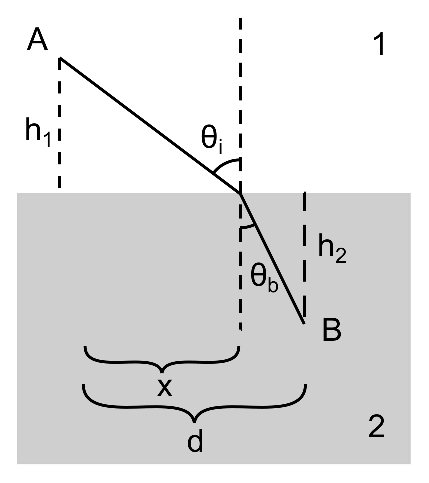
\includegraphics[scale=1]{./Images/refraction/refraction.eps}
	\caption{Illustration av brytning i en platt yta.}
	\label{fig:refraction}
\end{figure}
Tiden det tar för vågens strålgång att gå från $A$ till $B$ ges av
\begin{align*}
	t &= \frac{\sqrt{x^2 + h_1^2}}{c_1} + \frac{\sqrt{(d - x)^2 + h_1^2}}{c_2}.
\end{align*}
Derivatan med avseende på $x$ ges av
\begin{align*}
	\dv{t}{x} = \frac{x}{c_1\sqrt{x^2 + h_1^2}} - \frac{x - d}{c_2\sqrt{(d - x)^2 + h_1^2}}.
\end{align*}
Minimumet finns där derivatan är noll, vilket ger
\begin{align*}
	\frac{x}{c_1\sqrt{x^2 + h_1^2}} &= \frac{x - d}{c_2\sqrt{(d - x)^2 + h_1^2}} \\
	\frac{c_1}{c_2}                 &= \frac{\sqrt{(d - x)^2 + h_1^2}}{x - d}\frac{x}{\sqrt{x^2 + h_1^2}}.
\end{align*}
Trigonometrin ger
\begin{align*}
	\frac{c_1}{c_2} = \frac{1}{\sin{\theta_{\text{b}}}}\sin{\theta_{\text{i}}} = \frac{\sin{\theta_{\text{i}}}}{\sin{\theta_{\text{b}}}}.
\end{align*}

\paragraph{Villkor för totalreflektion}
\begin{align*}
	\theta_{\text{i}} = \arcsin{\frac{v_1}{v_2}}
\end{align*}

\deriv
Kommer direkt från brytningslagen när $\theta_{\text{i}} = \frac{\pi}{2}$.

\paragraph{Definitionen av reflektionskoefficient}
\begin{align*}
	R = \frac{I_\text{R}}{I_\text{I}}
\end{align*}
Subskriptet indikerar om det är intensiteten till den inkommande eller reflekterade vågen.

\paragraph{Definition av transmissionskoefficient}
\begin{align*}
	T = \frac{I_\text{T}}{I_\text{I}} = 1 - R
\end{align*}

\paragraph{Fassprang i gränsytor}
Om en våg går från ett medium med hög vågfart till ett med lägre, får den reflekterade vågen en fasförskjutning $\pi$. Om den går till ett medium med högre vågfart, har den reflekterade vågen samma fas.

\paragraph{Reflektionskoefficient för akustisk våg}
\begin{align*}
	R = \left(\frac{\abs{Z_1} - \abs{Z_2}}{\abs{Z_1} + \abs{Z_2}}\right)^2
\end{align*}

\paragraph{Transmissionskoefficient för akustisk våg}
\begin{align*}
	T = \left(\frac{2Z_1Z_2}{\abs{Z_1} + \abs{Z_2}}\right)^2
\end{align*}

\paragraph{Diffraktion från enkelt spalt}
\begin{align*}
	I = I_0I_0\left(\frac{\sin{\left(\frac{1}{2}ka\sin{\theta}\right)}}{\frac{1}{2}ka\sin{\theta}}\right)^2
\end{align*}
$a$ är spaltbrädden.

\deriv

\paragraph{Diffraktionsminima från enkelt spalt}
\begin{align*}
	a\sin{\theta} = m\lambda
\end{align*}

\deriv
En konsekvens formeln för intensitet vid diffraktion från enkelt spalt.

\paragraph{Diffraktion från flera spalter}
\begin{align*}
	I = I_0\frac{\sin^2{\left(\frac{1}{2}Nkd\sin{\theta}\right)}}{\sin{\left(\frac{1}{2}kd\sin{\theta}\right)}}
\end{align*}
$I_0$ är intensiteten från varje spalt, $N$ är antallet spalter, $d$ är avståndet mellan spalterna och $\theta$ är vinkeln observatören står i relativt normalen till gitteret.

\deriv
Varje källa har en vägskillnad $d\sin{\theta}$ relativt sin granne nedåt. Om man summerar vågorna får man
\begin{align*}
	s = \sum Ae^{i(kl - \omega t + (n -1)kd\sin{\theta})}
\end{align*}
för små $\theta$. Summeringen ger
\begin{align*}
	s &= Ae^{i(kl - \omega t)}\frac{1 - e^{iNkd\sin{\theta})}}{1 - e^{ikd\sin{\theta}}} \\
	  &= Ae^{i(kl - \omega t)}\frac{e^{-\frac{1}{2}iNkd\sin{\theta})}}{e^{-\frac{1}{2}ikd\sin{\theta}}}\frac{e^{\frac{1}{2}iNkd\sin{\theta}} - e^{-\frac{1}{2}iNkd\sin{\theta}}}{e^{\frac{1}{2}ikd\sin{\theta})} + e^{-\frac{1}{2}ikd\sin{\theta}}} \\
	  &= A\frac{e^{-\frac{1}{2}iNkd\sin{\theta})}}{e^{-\frac{1}{2}kd\sin{\theta}}}\frac{\sin{\left(\frac{1}{2}iNkd\sin{\theta}\right)}}{\sin{\left(\frac{1}{2}kd\sin{\theta}\right)}}e^{i(kl - \omega t)}.
\end{align*}
Den nya vågen har samma frekvens och våglängd, men en ny amplitud. Intensiteter beror på $\abs{A}^2$, vilket ger
\begin{align*}
	\frac{I}{I_0} = \frac{\sin^2{\left(\frac{1}{2}Nkd\sin{\theta}\right)}}{\sin^2{ \left(\frac{1}{2}kd\sin{\theta}\right)}}.
\end{align*}

\paragraph{Maxima vid diffraktion från flere spalter}
\begin{align*}
	d\sin{\theta} = m\lambda
\end{align*}

\deriv
Intensiteten vid flerstråleinterferens uppnår ett maximum när $\sin^2{\frac{1}{2}ikd\sin{\theta})} = 0$. Från detta kommer villkoret.

\paragraph{Första minimum vid diffraktion från en cirkulär spalt}
\begin{align*}
	\sin{\theta} = 1.22\frac{\lambda}{D}
\end{align*}
$D$ är spaltens diameter.

\paragraph{Braggs diffraktionslag}
\begin{align*}
	2d\sin{\theta} = m\lambda
\end{align*}
$d$ är separationen mellan atomplan i en kristall.

\deriv

\paragraph{Upplösning för gitter-baserat våglängdmätning}
\begin{align*}
	R = \frac{\lambda}{\Delta\lambda}
\end{align*}

\paragraph{Ljudabsorption}
\begin{align*}
	I = I_0e^{-\alpha x}
\end{align*}
Detta är ett sätt att beskriva energiförluster när vågen propagerar. $\alpha$ kallas för absorptionskoefficienten.

\paragraph{Vinkel för Mach-kon}
\begin{align*}
	\sin{\alpha} = \frac{c}{v_{\text{s}}}
\end{align*}
Om en ljudkälla rör sig med en fart $v_{\text{s}}$ som är snabbare än ljuden, kommer det bildas en så kallad Mach-kon bakom planet, där den inre vinkeln från källans bana till konens yta ges av denna ekvationen.

\deriv

\section{Modellering av systemer}
Syftet i denna delen är att diskutera systemer som kan modelleras med teorin bak klassiska vågor.

\subsection{Vätskor och gaser}
Vi tänker oss att vi trycker på vätskan eller gasen i en behållare med tvärsnittsarea $A$ och volym $V$. Detta får mediet att komprimeras. För $\dd{p} << p_0$ har man
\begin{align*}
	\dd{p} = -B\frac{\dd{V}}{V},
\end{align*}
där $B$ är mediets bulkmodul. Kompressionen kan tänkas få oändligt tunna volymelementer i mediet att förflytta sig ett avstånd $s(x)$, där $x$ är en koordinat som indikerar hur djupt i behållaren volymelementet är.

Betrakta nu vätskan eller gasen mellan två punkter $x$ och $x + \dd{x}$. Tryckskillnaden mellan dessa två punkterna ges av
\begin{align*}
	\dd{p} = -B\frac{\dd{V}}{V} = \dd{p} = -B\frac{A(s(x + \dd{x}) - s(x)}{A\dd{x}}\to -B\dv{s}{x}
\end{align*}

\section{Elektricitet}

\subsection{Ekvationer}

\paragraph{Definitionen av resistivitet}
\begin{align*}
	\rho = \frac{\abs{\vect{E}}}{\abs{\vect{J}}}
\end{align*}

\paragraph{Motstånd i en ledare}
\begin{align*}
	R = \frac{\rho L}{A}
\end{align*}

\paragraph{Seriekoppling av resistorer}
\begin{align*}
	R_\text{t} = \sum R_i
\end{align*}

\deriv

\paragraph{Parallellkoppling av resistorer}
\begin{align*}
	\frac{1}{R_\text{t}} = \sum \frac{1}{R_i}
\end{align*}

\deriv

\paragraph{Definitionen av kapacitans}
\begin{align*}
	C = \frac{Q}{V}
\end{align*}
$Q$ är beloppet av laddningen som lagras i kondensatorn (endast den positiva eller endast den negativa), och $V$ är spänningen som upprätthållas av kondensatorn.

\paragraph{Seriekoppling av kondensatorer}
\begin{align*}
	\frac{1}{C_\text{t}} = \sum\frac{1}{C_i}
\end{align*}

\deriv

\paragraph{Parallellkoppling av kondensatorer}
\begin{align*}
	C_\text{t} = \sum C_i
\end{align*}

\paragraph{Dielektrisk konstant}
\begin{align*}
	K = \frac{C}{C_0}
\end{align*}
$C_0$ betecknar kondensatorns kapacitans utan dielektrikum mellan plattarna. För en parallellplattkondensator har vi $K = \varepsilon_\text{r}$.

\paragraph{Kretser och elektromotiv kraft}
\begin{align*}
	V = \varepsilon - IR_\text{i}
\end{align*}
Den elektromotiva kraften $\varepsilon$ är spänningen som driver ström i kretsen. $R_\text{i}$ är kretsens inra motstånd, och då ges den faktiska spänningen i kretsen av denna formeln.

\deriv

\paragraph{Effektutveckling i en krets}
\begin{align*}
	P = VI
\end{align*}

\paragraph{Effektutveckling i resistiv komponent}
\begin{align*}
	P = I^2R = \frac{(\Delta V)^2}{R}
\end{align*}

\paragraph{Uppladdning av kondensator i RC-krets}
\begin{align*}
	&q = CV(1 - e^{-\frac{t}{RC}}), \\
	&I = \frac{V}{R}e^{-\frac{t}{RC}}
\end{align*}

\deriv

\paragraph{Utladdning av kondensator i RC-krets}
\begin{align*}
	&q = Q_0e^{-\frac{t}{RC}}), \\
	&I = -\frac{Q_0}{RC}e^{-\frac{t}{RC}}
\end{align*}

\subsection{Principer}

\section{Magnetism}

\subsection{Ekvationer}

\paragraph{Kraft på partikel i magnetfält}
\begin{align*}
	\vect{F} = q\vect{v}\times\vect{B}
\end{align*}

\paragraph{Flödet av magnetfält}
\begin{align*}
	\oint\vect{B}\cdot\dd{\vect{A}} = 0
\end{align*}

\paragraph{Cirkelbana för ladd partikel i magnetfält}
\begin{align*}
	R = \frac{mv}{\abs{q}B}
\end{align*}

\paragraph{Hastighetsfiltrering för vinkelrät elektriskt och magnetiskt fält}
\begin{align*}
	v = \frac{E}{B}
\end{align*}

\paragraph{Kraft på ledare i magnetfält}
\begin{align*}
	\dd{\vect{F}} = I\dd{\vect{l}}\vect{B}
\end{align*}

\paragraph{Magnetfält från laddning i rörelse}
\begin{align*}
	B = \frac{\mu_0q\vect{v}\times\vect{e}_{\vect{r}}}{4\pi r^2}
\end{align*}

\paragraph{Magnetfält kring ledare}
\begin{align*}
	\dd{B} = \frac{\mu_0I\dd{\vect{l}}\times\vect{e}_{\vect{r}}}{4\pi r^2}
\end{align*}

\paragraph{Ampères lag}
\begin{align*}
	\oint\limits_{\partial S}\vect{B}\cdot\dd{\vect{l}} = \mu_0\int\limits_{S}\vect{J}\cdot\dd{\vect{A}}
\end{align*}

\paragraph{Magnetfält kring oändlig ledare}
\begin{align*}
	B = \frac{\mu_0I}{2\pi r}
\end{align*}

\paragraph{Kraft per längd mellan två ledare}
\begin{align*}
	\frac{F}{L} = \frac{\mu_0I_1I_2}{2\pi r}
\end{align*}

\paragraph{Magnetfält i mitten av cirkulär ledare}
\begin{align*}
	B = \frac{\mu_0Ia^2}{2(x^2 + R^2)^\frac{3}{2}}
\end{align*}

\paragraph{Moment på kretsslinga i magnetfält}
\begin{align*}
	\vect{\tau} = \vect{\mu}\times\vect{B}
\end{align*}

\paragraph{Potensiell energi för kretsslinga i magnetfält}
\begin{align*}
	U = -\vect{\mu}\times\vect{B}
\end{align*}

\paragraph{Hall-effekt}
\begin{align*}
	nq = -\frac{J_xB_y}{E_z}
\end{align*}
$n$ representerar här tätheten av laddningsbärare.

\paragraph{Energi i en spola}
\begin{align*}
	U = \frac{1}{2}LI^2
\end{align*}

\paragraph{Energitäthet i magnetiska fält}
\begin{align*}
	u = \frac{B^2}{2\mu}
\end{align*}

\subsection{Principer}

\paragraph{Magnetiska dipoler}
Maxwells ekvationer förutspår att magnetism endast förekommer som dipoler.

\paragraph{Magnetiska material}
Elektroners bana och spinn ger upphov till magnetiska dipoler i material. I magnetiska material är dessa dipolerna i någon grad orienterade och ger upphov till ett makroskopiskt magnetiskt moment.

\section{Elektrodynamik}

\subsection{Ekvationer}

\paragraph{Maxwells ekvationer}
\begin{align*}
	&\oint_{\partial V}\vect{E}\cdot\dd{\vect{A}} = \frac{1}{\varepsilon_0}\int_{V}\dd{V}\rho, \\
	&\oint\vect{B}\cdot\dd{\vect{A}} = 0, \\
	&\oint_{\partial A}\vect{E}\cdot\dd{\vect{l}} = -\dv{\Phi_{B}}{t}, \\
	&\oint_{\partial A}\vect{B}\cdot\dd{\vect{l}} = \mu_0\left(\int_{A}\vect{J}\cdot\dd{\vect{A}} + \varepsilon\dv{\Phi_{E}}{t}\right).
\end{align*}
Man skulle kunna skriva en hel paragraf om varje ekvation för sig, men jag tyckte det blev snyggare att presentera de så här. $\Phi$ är flödet av fältet indikerat av subskriptet.

Den första ekvationen är Gauss' lag som vi känner den.

Den andra är Gauss' teorem för magnetfältet, även från statiken.

Den tredje ekvationen är Faradays lag. I praktiken betyder den att man kan inducera spänningar i kretsslingar.

Den fjärde ekvationen är Ampère-Maxwells lag, som även finns i statiken, men modifieras med en extra term.

\paragraph{Inducerad spänning i kretsslinga}
\begin{align*}
	\varepsilon = \oint(\vect{v}\times\vect{B})\cdot\dd{\vect{l}}
\end{align*} 

\subsection{Principer}



\section{Elektricitet}

\subsection{Ekvationer}

\paragraph{Effektutveckling i en krets}
\begin{align*}
	P = VI
\end{align*}

\paragraph{RMS-ström- och spänning}
\begin{align*}
	I_{\text{rms}} = \sqrt{\expval{I}},\ V_{\text{rms}} = \sqrt{\expval{V}}
\end{align*}
I en sinusoidal krets har man
\begin{align*}
	I_{\text{rms}} = \frac{I_{\text{max}}}{\sqrt{2}}
\end{align*}
och motsvarande för spänningen.

\paragraph{Ohms lag}
\begin{align*}
	V = ZI
\end{align*}

\paragraph{Definitionen av resistivitet}
\begin{align*}
	\rho = \frac{\abs{\vect{E}}}{\abs{\vect{J}}}
\end{align*}

\paragraph{Motstånd i en ledare}
\begin{align*}
	R = \frac{\rho L}{A}
\end{align*}

\paragraph{Seriekoppling av resistorer}
\begin{align*}
	R_\text{t} = \sum R_i
\end{align*}

\deriv

\paragraph{Parallellkoppling av resistorer}
\begin{align*}
	\frac{1}{R_\text{t}} = \sum \frac{1}{R_i}
\end{align*}

\deriv

\paragraph{Effektutveckling i resistiv komponent}
\begin{align*}
	P = I^2R = \frac{(\Delta V)^2}{R}
\end{align*}

\paragraph{Definitionen av kapacitans}
\begin{align*}
	C = \frac{Q}{V}
\end{align*}
$Q$ är beloppet av laddningen som lagras i kondensatorn (endast den positiva eller endast den negativa), och $V$ är spänningen som upprätthållas av kondensatorn.

\paragraph{Impedans i en kondensator}
\begin{align*}
	Z = i\frac{1}{\omega C}
\end{align*}

\paragraph{Seriekoppling av kondensatorer}
\begin{align*}
	\frac{1}{C_\text{t}} = \sum\frac{1}{C_i}
\end{align*}

\deriv

\paragraph{Parallellkoppling av kondensatorer}
\begin{align*}
	C_\text{t} = \sum C_i
\end{align*}

\paragraph{Dielektrisk konstant}
\begin{align*}
	K = \frac{C}{C_0}
\end{align*}
$C_0$ betecknar kondensatorns kapacitans utan dielektrikum mellan plattarna. För en parallellplattkondensator har vi $K = \varepsilon_\text{r}$.

\paragraph{Kretser och elektromotiv kraft}
\begin{align*}
	V = \varepsilon - IR_\text{i}
\end{align*}
Den elektromotiva kraften $\varepsilon$ är spänningen som driver ström i kretsen. $R_\text{i}$ är kretsens inra motstånd, och då ges den faktiska spänningen i kretsen av denna formeln.

\deriv

\paragraph{Uppladdning av kondensator i RC-krets}
\begin{align*}
	&q = CV(1 - e^{-\frac{t}{RC}}), \\
	&I = \frac{V}{R}e^{-\frac{t}{RC}}
\end{align*}

\deriv

\paragraph{Utladdning av kondensator i RC-krets}
\begin{align*}
	&q = Q_0e^{-\frac{t}{RC}}), \\
	&I = -\frac{Q_0}{RC}e^{-\frac{t}{RC}}
\end{align*}

\deriv

\paragraph{Uppladdning av spola i RL-krets}
\begin{align*}
	I = \frac{V}{R}\left(1 -e^{-\frac{R}{L}t}\right)
\end{align*}

\deriv

\paragraph{Utladdning av spola i RL-krets}
\begin{align*}
	I = I_0e^{-\frac{R}{L}t}
\end{align*}

\paragraph{Impedans i en spola}
\begin{align*}
	Z = i\omega L
\end{align*}

\paragraph{Fasvinkel i AC-krets}
\begin{align*}
	\tan{\theta} = \frac{\omega L - \frac{1}{\omega C}}{R}
\end{align*}

\paragraph{Medeleffekt i AC-krets}
\begin{align*}
	\expval{P} = V_{\text{rms}}I_{\text{rms}}\cos{\phi}
\end{align*}

\paragraph{Egenfrekvens i LC-krets}
\begin{align*}
	\omega = \sqrt{\frac{1}{LC}}
\end{align*}

\paragraph{Dämpningskriterie för RLC-krets}
\begin{align*}
	\frac{R^2}{4L^2} - \frac{1}{LC} < 0
\end{align*}

\deriv
Kan vara fel.

\paragraph{Egenfrekvens i underdämpad RLC-krets}
\begin{align*}
	\omega ' = \sqrt{\frac{1}{LC} - \frac{R^2}{4L^2}}
\end{align*}

\deriv

\paragraph{Spänningsrelation i transformator}
\begin{align*}
	\frac{V_2}{V_1} = \frac{N_2}{N_1}
\end{align*}

\paragraph{Spänningsrelation för transformator med motstånd}
\begin{align*}
	\frac{V_1}{I_1} = \frac{R}{\left(\frac{N_2}{N_1}\right)^2}
\end{align*}

\paragraph{Korrigerad medelström i ett galvanometer}
\begin{align*}
	I_{\text{rav}} = \frac{2}{\pi}I_{\text{max}}
\end{align*}
Med rätt kretsuppsätt ger detta strömmen i galvanometeret så att i löpet av en cykel får man samma laddningsflöde i galvanometeret som om den konstanta strömmen $I_{\text{rav}}$.

\subsection{Principer}

\section{Elektromagnetiska vågor}
Från Maxwells ekvationer kan man visa att flera storheter kopplade till elektromagnetism följer vågekvationen. Dessa vågor kallas för elektromagnetiska vågor. Experimenter visade att ljus propagerade med samma farten som den teoretiska farten till elektromagnetiska vågor, och därmed blev det snabbt etablerat att ljus är elektromagnetiska vågor. Därmed kommer vi ägna en hel sektion åt att diskutera de.

\subsection{Principer}

\paragraph{Essensiell information från Maxwells ekvationer}
Från Maxwells ekvation får man veta att
\begin{itemize}
	\item elektromagnetiska vågor är transversella.
	\item elektromagnetiska vågor utbredar sig med ljusfarten $c = \frac{1}{\sqrt{\varepsilon_0\mu_0}}$ i vakuum, och motsvarande i andra media.
	\item $\vect{B}\perp\vect{E}$.
	\item $B = \frac{1}{c}E$.
	\item $\vect{E}\times\vect{B}$ pekar i utbridningsriktningen.
\end{itemize}

\paragraph{Dispersion}
Dispersion är när ett mediums brytningsindex beror på vågens våglängd.

\paragraph{Polarisation}
Elektriskt och magnetiskt fält är vektorstorheter, och det betyder att de kan svänga i olika plan. Ljusets polarisation refererar till hur fälterna svängar i planet normalt på utbridgningen.

Ljus kan vara
\begin{itemize}
	\item linjärpolariserat, så att fältet oscillerar på en linje i det normala planet.
	\item elliptiskt polariserat, så att fältet oscillerar på en ellips i det normala planet.
	\item opolariserat, så att fältet oscillerar godtyckligt utan preferens för någon riktning.
\end{itemize}

\subsection{Ekvationer}

\paragraph{Vågekvationen för $\vect{E}$}
\begin{align*}
	\laplacian{\vect{E}} = \varepsilon\mu\pdv{\vect{E}}{t}
\end{align*}

\deriv

\paragraph{Definitionen av brytningsindex}
\begin{align*}
	n = \frac{c_0}{c}
\end{align*}
Här är $c_0$ ljusfarten i vakuum. Per definition är $n\geq 1$ i linjära materialer. Definitionen ger
\begin{align*}
	n = \sqrt{\varepsilon_{\text{r}}\mu_{\text{r}}}
\end{align*}
där $\varepsilon_{\text{r}}, \mu_{\text{r}}$ är relativa permeabiliteter och permittiviteter.

\paragraph{Reflektionskoefficient för elektromagnetiska vågor}
\begin{align*}
	R = \left(\frac{n_1 - n_2}{n_1 + n_2}\right)^2
\end{align*}

\paragraph{Våglängd i medium}
\begin{align*}
	\lambda = \frac{\lambda_0}{n}
\end{align*}
$\lambda_0$ är våglängden i vakuum. En direkt konsekvens av detta är att
\begin{align*}
	k = nk_0
\end{align*}
för vågvektorn, där $k_0$ är vågvektorns längd i vakuum.

\deriv
Vi har från innan att vid transmission mellan två medier ändras inte frekvens. Detta ger att
\begin{align*}
	\lambda = \frac{c}{f} = \frac{c_0}{nf} = \frac{\lambda_0}{n}
\end{align*}
där $c_0$ är vågfarten i vakuum.

\paragraph{Definitionen av optisk väg}
För en given bana definieras den optiska vägen ljus tar som
\begin{align*}
	L = \int\limits_{C}\dd{l}n,
\end{align*}
som för materialer med konstant brytningsindex reduceras till
\begin{align*}
	L = \sum L_in_i,
\end{align*}
där $L_i$ är sträckan vägen rör sig i materialet med brytningsindex $n_i$.

\paragraph{Poyntingvektorn}
\begin{align*}
	\vect{S} = \frac{1}{\mu_0}\vect{E}\times\vect{B}
\end{align*}
Poyntingvektorn ger information om energitransport från en elektromagnetisk våg. Dens riktning indikerar i vilken riktning energin transporteras, och dens belopp indikerar hur mycket energi som transporteras.

\deriv
I ett litet tidsintervall flödar energin
\begin{align*}
	\dd{U} = u\dd{V} = uAc\dd{t}
\end{align*}
genom arean $A$. För en elektromagnetisk våg har man
\begin{align*}
	u = \frac{1}{2}\varepsilon_0E^2 + \frac{1}{2\mu_0}B^2.
\end{align*}
Med relationen $B = \frac{E}{c}$ får man
\begin{align*}
	u = \varepsilon_0E^2,
\end{align*}
vilket ger
\begin{align*}
	\dd{U} = u\dd{V} = \varepsilon_0E^2Ac\dd{t}.
\end{align*}
Flödet per tidsenhet och area ges av
\begin{align*}
	S = \frac{1}{A}\dv{U}{t} = \frac{EB}{\mu_0}.
\end{align*}
Givet detta, definierar man
\begin{align*}
	\vect{S} = \frac{1}{\mu_0}\vect{E}\times\vect{B}
\end{align*}
som uppfyller
\begin{align*}
	\abs{\vect{S}} = \frac{EB}{\mu_0}
\end{align*}
och vars riktning även ger information om i vilken riktning energin transporteras.

\paragraph{Intensitet för elektromagnetisk våg}
\begin{align*}
	I = \frac{1}{2}\varepsilon_0cE^2
\end{align*}

\deriv'
Enligt definitionen är
\begin{align*}
	I = \expval{S}
\end{align*}

\section{Optik}

\subsection{Principer}

\paragraph{Huvudplan och fokalplan}
Betrakta figur \ref{fig:optical_planes}.
\begin{figure}[!ht]
	\centering
	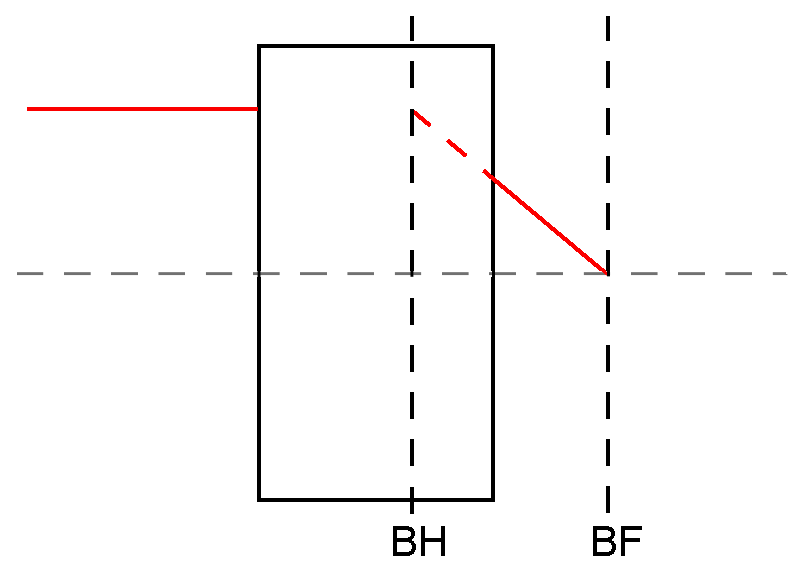
\includegraphics[scale=0.8]{./Images/optical_planes/optical_planes.eps}
	\caption{Illustration av bakra huvdudplan och fokalplan för ett godtyckligt optiskt system.}
	\label{fig:optical_planes}
\end{figure}

Lådan illustrerar ett optiskt system. Den röda strålen representerar strålgången. Det bakra fokalplanet, märkt BF, är planet där en parallell stråle skär den gråa centrallinjen och som är normalt på centrallinjen. Det bakra huvudplanet, märkt BG, är planet så att det optiska systemets verkan på strålan är ekvivalent med att all brytning sker i det planet, som illustrerat. Det fremre fokalplanet och huvudplanet fås på analogt sätt om man betraktar en stråle som kommer från höger.

\paragraph{Fokalavstånd}
Fokalavståndet till ett optisk system är avståndet från systemets bakre huvudplan till dets bakre fokalplan.

\paragraph{Konvexa och konkava linser}
En konvex linsa samlar parallela strålar, medan en konkav lins sprider parallella strålar.

\subsection{Ekvationer}

\paragraph{Reflektionslagen för plana speglar}
\begin{align*}
	s = -s'
\end{align*}
Alternativt, i kartesisk konvention:
\begin{align*}
	s = s'.
\end{align*}

\paragraph{Spegelekvationen för sfärisk spegel}
\begin{align*}
	\frac{1}{s} + \frac{1}{s'} = \frac{2}{R}
\end{align*}
Alternativt, i kartesisk konvention:
\begin{align*}
	-\frac{1}{s} + \frac{1}{s'} = \frac{2}{R}
\end{align*}
$R$ är spegelns krökningsradie.

\deriv

\paragraph{Brytning i sfäriska ytor}
\begin{align*}
	\frac{n_1}{s} + \frac{n_2}{s'} = \frac{n_2 - n_1}{R}
\end{align*}
Alternativ, i kartesisk konvention:
\begin{align*}
	-\frac{n_1}{s} + \frac{n_2}{s'} = \frac{n_2 - n_1}{R}.
\end{align*}

\deriv

\paragraph{Linsformeln för tunna linser}
\begin{align*}
	\frac{1}{s} + \frac{1}{s'} = \frac{1}{f}
\end{align*}

\deriv

\paragraph{Linsformeln för krökt lins}
\begin{align*}
	\frac{1}{s} + \frac{1}{s'} = \left(\frac{n_2}{n_1} - 1\right)\left(\frac{1}{R_1} - \frac{1}{R_2}\right)
\end{align*}

\section{Teckenkonvention i optik}
Utseendet till ekvationerna vi användar i optik ska beror på teckenkonventionen man användar. En möjlighet är att använda kartesisk teckenkonvention. Denna baseras på att
\begin{itemize}
	\item allt ljus kommer från höger mot vänster.
	\item Koordinatsystemet definieras med origo i centrum av den optiska komponenten, $x$-axeln med positiv riktning mot höger och $y$-axeln med positiv riktning uppåt.
\end{itemize}
Detta implicerar följande konvention:
\begin{table}[!ht]
	\makebox[\textwidth][c]
	{\begin{tabular}{| l | l | l |}
		\hline
		            & + & - \\
		\hline
		Objektavstånd         & Objekt till höger om optisk objekt & Objekt till vänster om optisk objekt \\
		\hline
		Bildavstånd           & Bild till höger om optisk objekt   & Bild till bänster om optisk objekt \\
		\hline
		Fokallängd för lins   & Samlar ljus till höger (konvex)    & Samlar ljus till vänster (konkav) \\
		\hline
		Fokallängd för spegel & Centrum till höger (konvex)        & Centrum till vänster (konkav) \\
		\hline
	\end{tabular}}
\end{table}

%Räkna på sfärisk yta

Alternativt kan man använda den så kallade "Real Is Positive"- konventionen (R.I.P) som används i kurslitteraturen. Denna definieras av följande tabell:
\begin{table}[!ht]
	\makebox[\textwidth][c]
	{\begin{tabular}{| l | l | l |}
		\hline
		            & + & - \\
		\hline
		Objektavstånd för linser       & Objekt till vänster om lins     & Objekt till höger om lins \\
		\hline
		Bildavstånd för linser         & Bild till höger om lins         & Bild till vänster om lins \\
		\hline
		Fokallängd för lins            & Samlar ljus till höger (konvex) & Samlar ljus till vänster (konkav) \\
		\hline
		Objektavstånd för speglar      & Objekt till vänster om spegel   & Objekt till höger om spegel \\
		\hline
		Bildavstånd för speglar        & Bild till vänster om spegel     & Bild till höger om spegel \\
		\hline
		Fokallängd för spegel          & Centrum till vänster (konkav)   & Centrum till höger (konvex) \\
		\hline
		Objektavstånd för sfärisk yta  & Objekt till vänster om yta      & Objekt till höger om yta \\
		\hline
		Bildavstånd för sfärisk yta    & Bild till höger om spegel       & Bild till vänster om yta \\
		\hline
		Krökningsradie för sfärisk yta & Centrum till höger              & Centrum till vänster \\
		\hline
	\end{tabular}}
\end{table}

Varför en konvention är klart överlegen är triviellt och lämnas som en övning till läsaren.

\end{document}
